%intro (motivation and outline)
% about pixel-based vs voxel-based for incremental reconstruction
While incremental reconstruction with PNN is fast, it has its shortcomings. Due to the simplicity of the algorithm, the quality of the reconstructed volume is not as good as can be obtained with voxel-based methods using interpolation. Furthermore, hole filling is problematic when aiming for real-time performance. What is desired is a method that have high hole-free reconstruction quality, that can preferably be adjusted for a quality-time tradeoff, and one that is suitable for incremental updates of the volume without processing all voxels.

Pixel-based methods have the advantage of processing only the voxels that is actually updated by each b-scan, but the simplest variants can have the problem of holes. More advanced voxel-based methods can offer high reconstruction quality without holes, but are unsuitable for incremental updates. The method presented in this section combines the advantages from both approaches. The steps taken will be explained, together with issues from implementation and parallelization of the method are also covered.

% description of steps in the algorithm (incl DW and PT)
\subsection{Method}

% steps:
	% find ray-plane intersections
		% construct rays along axis and perform ray-plane intersection calculations
		% convert intersections to volume indices
	% fill voxels between intersection indices
		% linear interpolation ("DW") \cite{trobaugh1994}
			% for each b-scan in window:
				% orthogonal project voxel on b-scan
				% bilinear interpolation of 4 pixels
				% weight by inverse distance
			% divide by sum of weights
		% PT \cite{coupe2005}
			% linearly interpolate timetags by orthogonal distance
			% cubic interpolate 4 plane equations by key function
			% convert voxel coordinates on virtual plane to pixel indices
			% bilinear interpolate of 4 pixels on each b-scan
			% weight by inverse distance and divice by sum of weights
		% compound

The essence of the method is to transform incoming b-scan planes into the volume, but also to only process voxels located \emph{between} b-scans. For the voxels processed, voxel-based interpolation methods can be used to fill their values. This is what is meant by combining the pixel- and voxel-based approaches (or rather, the forward and backward approaches). B-scans are processed forwardly into the volume, but instead of filling the volume directly from the pixels, voxels between inserted b-scans have their values interpolated from the surrounding b-scans.

	\begin{figure}[h]
	\centering
	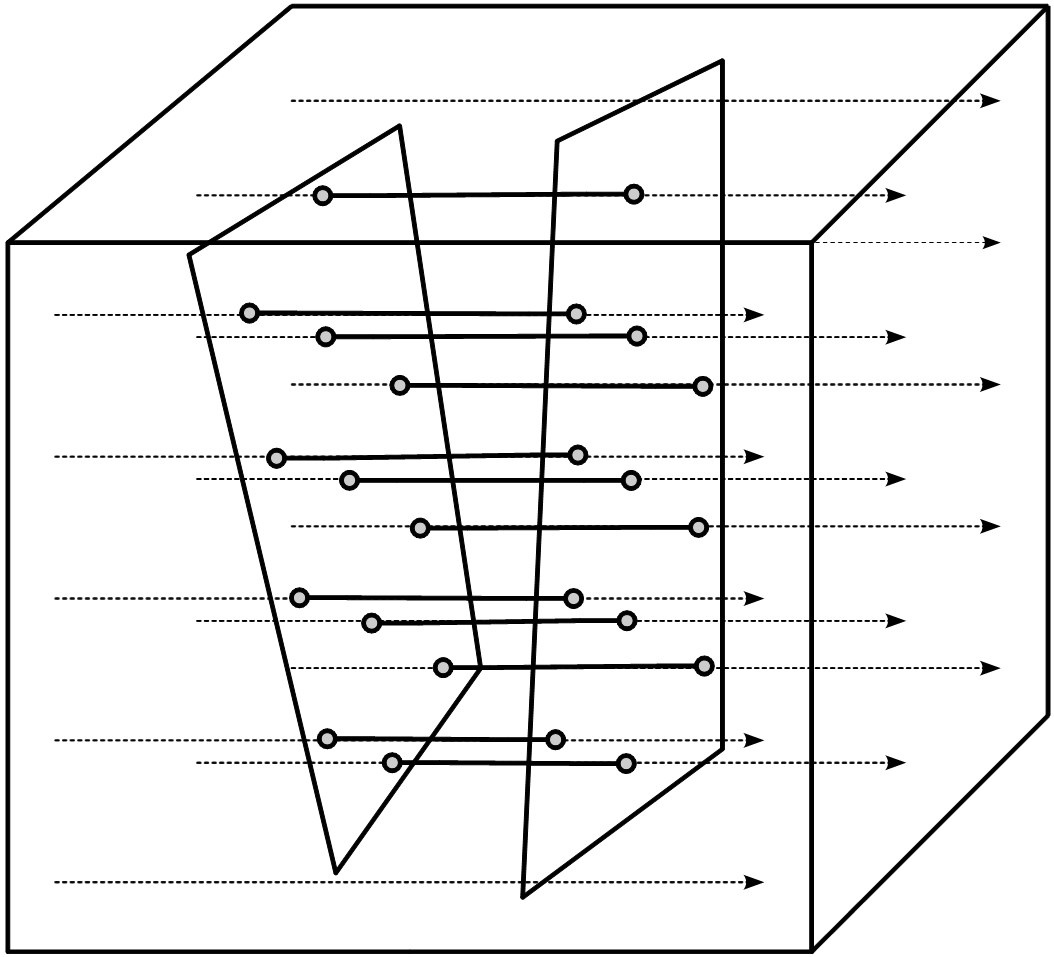
\includegraphics[height=0.4\textheight]{graphics/trace_intersections.png}
	\caption{Finding voxels between b-scans}
	\label{fig:trace_intersections}
	\end{figure}

For each incoming b-scan, we transform its corner points using the tracking data and construct its plane equation as previously described in Section \ref{section:non-incremental_vnn}. Figure \ref{fig:trace_intersections} show how the voxels between the current and previous b-scans are calculated. First, rays are constructed along columns of voxels, starting at the edge of the volume with one ray per column. These rays are used for ray-plane intersection calculations with the current and previous b-scan planes. The distance $t$ along a ray starting at $r_0$ with direction $r_d$ to a plane with equation parameters $(a,b,c,d)$ is given by Equation \ref{eq:ray-plane0}, and the voxel indices $(x,y,z)$ are given by Equation \ref{eq:ray-plane1}. Each ray gives one intersection point with the current b-scan, and another with the previous b-scan. The voxels between these will lie next to each other.

\begin{equation}
	\label{eq:ray-plane0}
	t = -\frac{(a,b,c) \cdot r_0 + d}{(a,b,c) \cdot r_d}
\end{equation}

\begin{equation}
	\label{eq:ray-plane1}
	(x,y,z) = \frac{r_0 + tr_d}{\Delta v}
\end{equation}

After the voxels between the b-scans have been found, they are each filled using a voxel based method. In our system, one can choose between two methods: one based on distance weighted orthogonal projections, and one based on cubic interpolation of the probe trajectory.

\subsubsection{Distance Weighted Orthogonal Projections}

	This method builds on the approach described by Trobaugh \textit{et al.}\ \cite{trobaugh1994}, where each voxel filled is orthogonally projected onto nearby b-scans and interpolated using the distance to the b-scan planes. But while Trobaugh \textit{et al.}\ project onto only two surrounding b-scans, we project onto the $n_w \leq n$ b-scans surrounding the voxel. The number of b-scans ($n_w$) taken into account for each voxel can be adjusted for a tradeoff between quality and performance. The 2D coordinates of the projected point on the b-scan plane can be found using equations previously described in Section \ref{section:non-incremental_vnn}. What differs, however, is that we project not only to the closest b-scan, but to all nearby b-scans. The number of b-scans used for each voxel increases the quality.  For each projection, the pixel intensity is given by a bilinear interpolation of the 4 pixels closest to the projected coordinates, as shown in Figure \ref{fig:bilinear} and given by Equation \ref{eq:bilinear_eq} where $x_f$ and $y_f$ is a fraction between 0.0 and 1.0 that says how far the projected point is from the closest pixel coordinates to the top-left. E.g.\ 0.5 means halfway between $(x,y)$ and $(x+1,y+1)$ (see figure). If one or more of the pixels are outside the ROI, the bilinear interpolated intensity is not used. Each intensity used is weighted by the inverse of the distance to the b-scan plane given by Equation \ref{eq:distance}. To normalize the result, it is divided by the sum of the weights as given by Equation \ref{eq:weighting}.
	
	\begin{figure}[h]
	\centering
	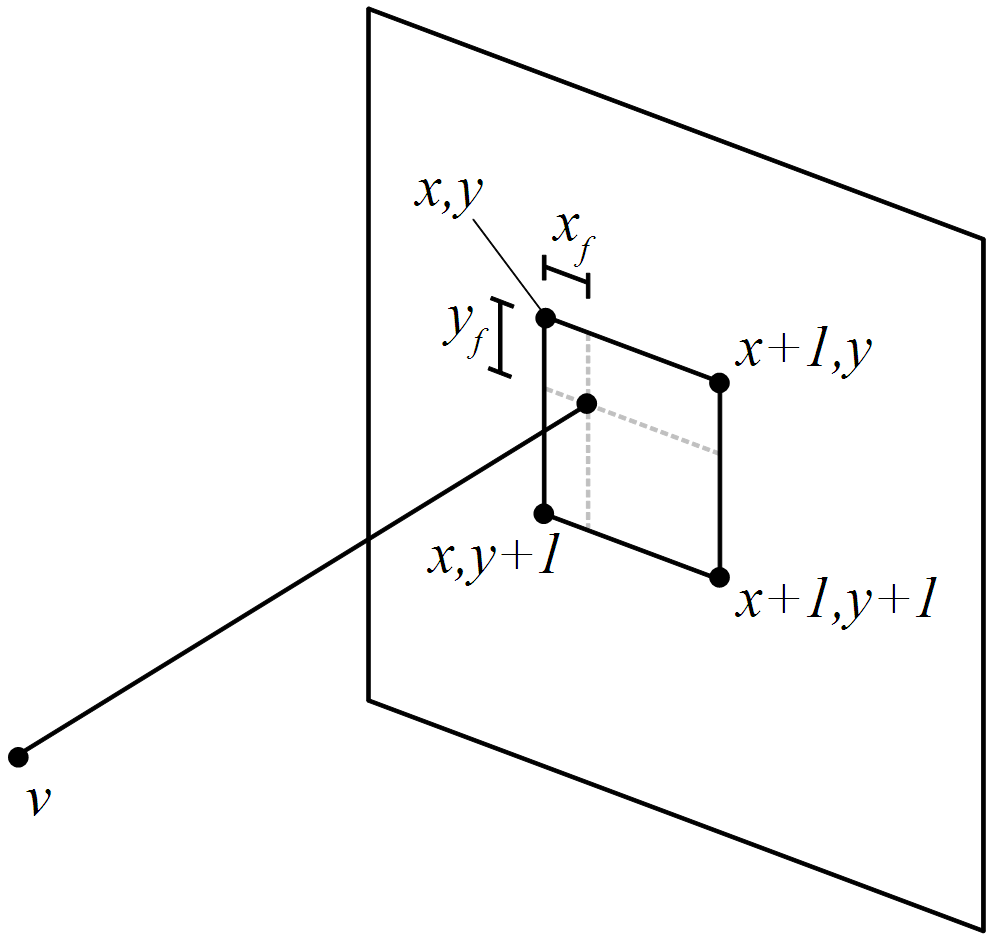
\includegraphics[height=0.35\textheight]{graphics/bilinear.png}
	\caption{Bilinear interpolation}
	\label{fig:bilinear}
	\end{figure}
	
	\begin{eqnarray}
		bilinear 	& = & b\-scan(x,y)(1-x_f)(1-y_f) + \nonumber \\
					&	& b\-scan(x+1,y) x_f (1-y_f) + \nonumber \\
					&	& b\-scan(x,y+1)(1-x_f) y_f + \nonumber \\
					&	& b\-scan(x+1,y+1) x_f y_f
		\label{eq:bilinear_eq}
	\end{eqnarray}
	
	\begin{equation}
		\label{eq:weighting}
		value_{dwop} = \frac{\sum_i (bilinear_i \cdot weight_i)}{\sum_i weight_i}
	\end{equation}
	
\subsubsection{Cubic Interpolation of Probe Trajectory}

	% linearly interpolate timetags by orthogonal distance
	% cubic interpolate 4 plane equations by key function
	% convert voxel coordinates on virtual plane to pixel indices
	% bilinear interpolate of 4 pixels on each b-scan
	% weight by inverse distance and divice by sum of weights
	
	This method is based on reconstruction as described by Coupe \textit{et al.}\ \cite{coupe2005}, but performed only on the voxels between two b-scans. The principle is to perform cubic interpolation of the tracking data as an estimation of the trajectory of the ultrasound probe. First, the timetags of two adjacent b-scans are linearly interpolated based on the orthogonal distance from the voxel coordinates in space to the b-scan planes, as illustrated in Figure \ref{fig:virtual_timetag} and given in Equation \ref{eq:virtual_timetag}. This new timetag is called a \emph{virtual timetag} and belongs to a virtual plane going through the voxel.
	
	\begin{figure}[h]
	\centering
	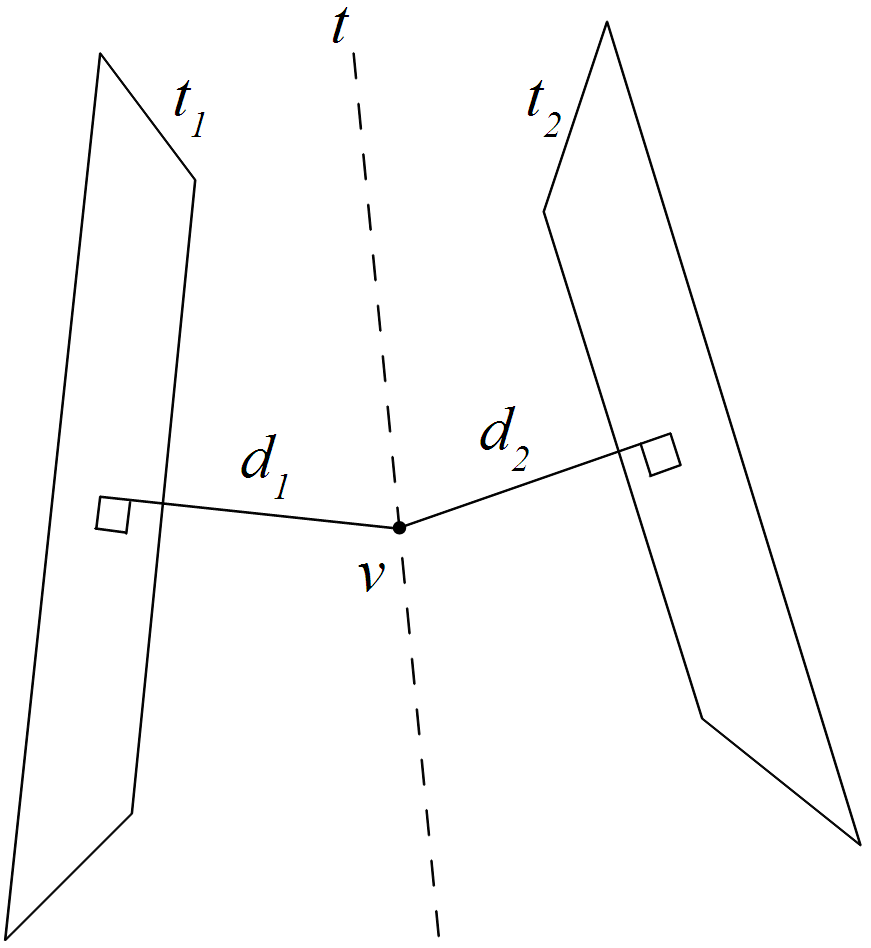
\includegraphics[height=0.35\textheight]{graphics/virtual_timetag.png}
	\caption{Timetag of virtual plane}
	\label{fig:virtual_timetag}
	\end{figure}
	
	\begin{equation}
		\label{eq:virtual_timetag}
		t = \frac{d_2 t_1}{d_1+d_2} + \frac{d_1 t_2}{d_1+d_2}
	\end{equation}
	
	To find the plane equation, top-left corner and x and y-vectors of the b-scan in the virtual plane, we use cubic interpolation based on the timetags through the \emph{key function} given in Equation \ref{eq:key_function} with $a = -\frac{1}{2}$. We interpolate plane equation parameters, corner and vector coordinates from four adjacent b-scans, where the two internal b-scans are those previously used to interpolate the virtual timetag. The cubic interpolation is shown in Figure \ref{fig:cubic_interpolation}. For each parameter or coordinate $\alpha$ to interpolate, the value of the key function is used in Equation \ref{eq:cubic_interpolation}.
	
	\begin{figure}[h]
	\centering
	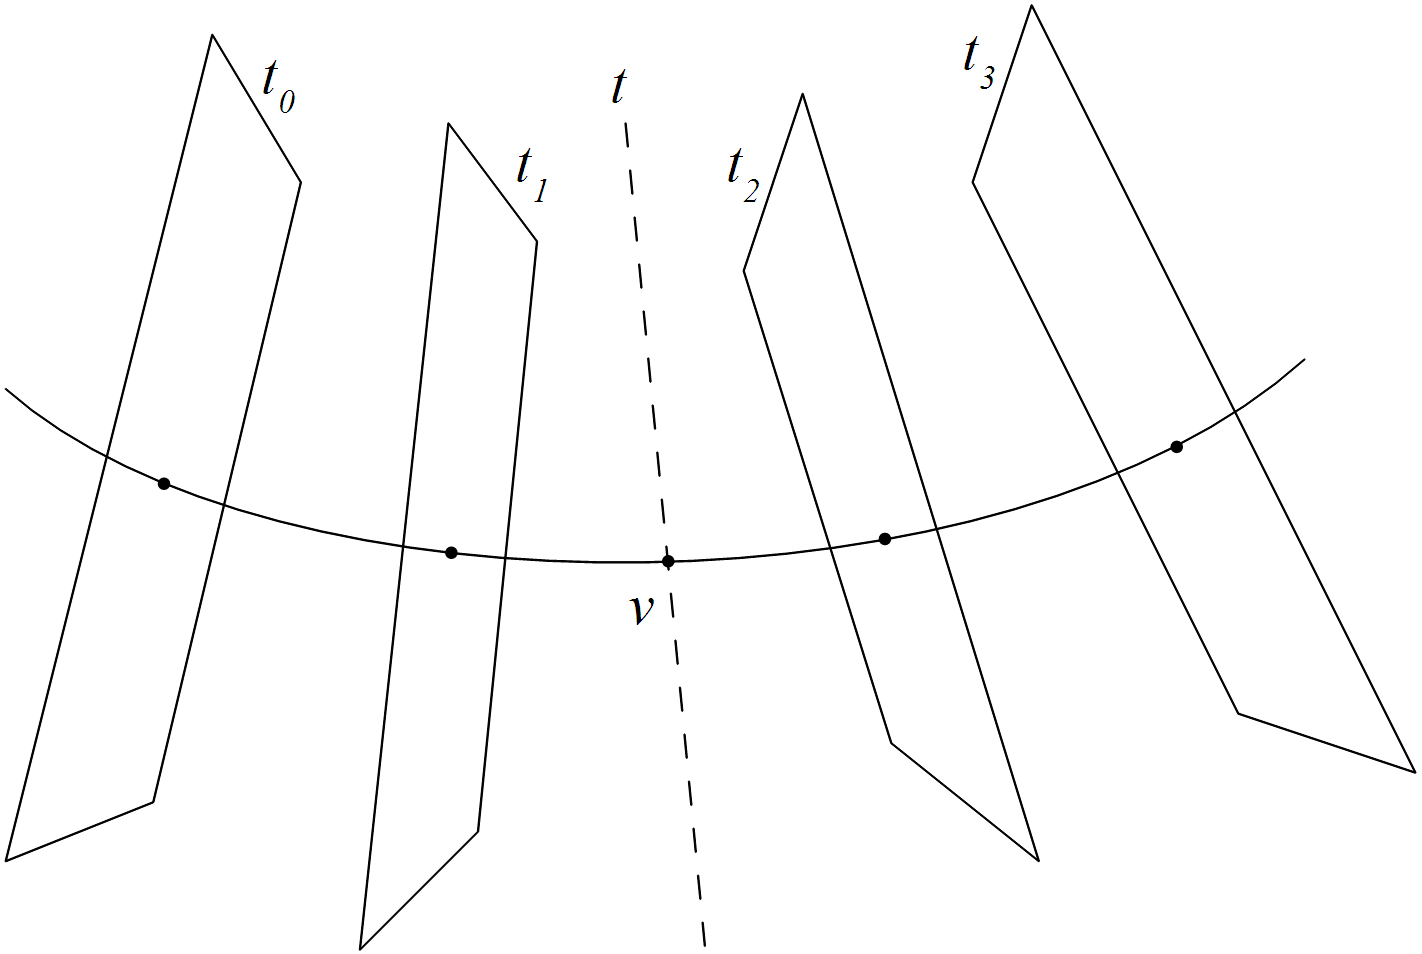
\includegraphics[height=0.35\textheight]{graphics/cubic_interpolation.png}
	\caption{Cubic interpolation of four b-scans}
	\label{fig:cubic_interpolation}
	\end{figure}
	
	\begin{equation}
		\label{eq:key_function}
		\phi(\beta) = \left\{ 
			\begin{array}{l l}
				(a+2)\beta^3 - (a+3)t^2 + 1 			& \quad \mbox{if $0 \leq \beta < 1$} \\
				a\beta^3 - 5a\beta^2 + 8a\beta - 4a 	& \quad \mbox{if $1 \leq \beta < 2$} \\
				0 										& \quad \mbox{if $2 \leq \beta$} \\
			\end{array}
		\right.
	\end{equation}
	
	\begin{equation}
		\label{eq:cubic_interpolation}
		\alpha = \sum_{i=0}^{4}\alpha_i \phi(\left|\frac{t-t_i}{t_1-t_0}\right|)
	\end{equation}
	
	When the virtual plane has been obtained, the 2D coordinates of the voxel (lying on the plane) can be found using the equations described in Section \ref{section:non-incremental_vnn}. These coordinates are then used on each of the four adjacent b-scans, and the pixels at those locations are bilinearly interpolated using Equation \ref{eq:bilinear_eq}. The four bilinearly interpolated values are then weighted by the inverse orthogonal distance to each b-scan from the voxel coordinates according to Equation \ref{eq:weighting}.

% description of how algorithm is implemented and parallelized
\subsection{Implementation and Parallelization}
	\label{section:incr_hq_impl}
	% queues and windows (options for plane a and b)
	% choose axis
	% restart if difference in timetags > cutoff
	% NDRange
	% CPU/GPU distribution
	
	Code listings of the implemented OpenCL kernels can be found in Appendix \ref{section:incremental_kernel}. To be able to interpolate between several b-scans, one solution is to queue up a buffer of incoming b-scans and tracking data. As incoming data is pushed into the queue, data is popped from the other end of the queue. When the session begins, the queue is simply filled without processing any of the input. During the session, this queue will be a "sliding window" across the stream of incoming data. The number of b-scans (each with associated tracking data) in the window is at least four if the probe trajectory (PT) method is used to fill the voxels, and a number $n_w \leq n$ if distance weighted orthogonal projections (DWOP) is used. There are several options for which two b-scan planes to use in the window when finding voxels to fill between them. To avoid repeated fillings of the same voxels, we use the planes of the two b-scans in the center of the window.
	
	When constructing the rays for the ray-plane intersection calculations, any axis can be used as a direction for the rays. As we parallelize with one thread per ray, we want to distribute work as evenly as possible. This means choosing an axis that is the most orthogonal to the normal for each b-scan. And by this we mean the axis that has the lowest angle between itself and the normalized b-scan plane normal $\bb{n}$ as given in Equation \ref{eq:axis}. The axis used is re-evaluated for each incoming b-scan.

\begin{equation}
	\label{eq:axis}
	S = \{(0,0,1), (0,1,0), (1,0,0)\}, \;\; ARGMIN_{\bb{a}\in S}(\bb{a} \cdot \bb{n})
\end{equation}

	To handle discontinuities in the input stream (e.g.\ from pauses in tracking during one session), a check is made for each incoming b-scan. If the increase in time according to the timetags is above a cutoff value, the reconstruction is restarted from that b-scan instead of attempting to interpolate across the discontinuity. Ultrasound systems usually have a regular acquisition rate $f$, and so a cutoff at $\frac{2}{f}$ is sufficient.
	
	As mentioned, the computations are parallelized with one thread per ray, and this \textit{NDRange} is kept as the voxels found by one ray will also be processed by the same thread. Assuming that the z-axis is always used as the best axis, the \textit{NDRange} will be $w \times h$ threads, each processing a number of voxels between 1 and the highest separation between two adjacent b-scans (typically $\leq 5$). 